\chapter{Field data collection}
\label{txt:odk}
\index{Field data collection}
\index{ODK}

 Accurate field notes are essential to ensure the greatest value is made of samples.  With no metadata associated with a sample, it is of little more use than firewood.  At the same time, though, time in the field is often very limited therefore there is pressure to record metadata as efficiently as possible.
 
 Dendro field data collection is traditionally done through either handwritten field notebooks or paper forms. The trade-off between comprehensive metadata collection and time efficiency means that fieldnotes are often abbreviated with the best intentions to write them up fully in the evening or on the return to the laboratory.  These sorts of pressures typically lead to the bare minimum of metadata being recorded.
 
 In Tellervo, one solution to this problem makes use of the collection of open source tools known as Open Data Kit (ODK).  ODK is a platform that utilises (Android) mobile phones and tablets as simple field data collection devices.  It was originally designed to collect medical information in rural regions of developing countries and has proven to be extremely effective and reliable.  Forms are designed and uploaded to the mobile device, and a simple sequence of questions enables the field researcher to enter text, categorical, numerical, GPS and photographic data.  On return to base, the data is then uploaded from the device to a database for analysis.  The system does not rely on mobile network signals that are typically weak or non-existent in remote field regions, rather storing the data on the device and then transfering the data at the end of the day once the researcher returns to base.
 
 The hardware requirements for the mobile application are very low meaning it can run on entry level phones and tablets.  The addition of rugged waterproof cases mitigates for difficult field conditions, and the storage of data on removeable flash memory cards means that data can often be recovered even when disaster strikes your device.  Entering data via touch screens is now second nature to most people, enabling data entry speeds approaching or exceeding that of a traditional keyboard.
 
 The field data collection system implemented in Tellervo is described in the following sections and by \citet{brewer2016}.
 
 
 \section{Data transfer}
 There are two methods of transferring data from ODK mobile devices to the Tellervo database.  The first and most convenient is via wifi and/or cellular network connections directly to the Tellervo server.  This is quick and effective, however, it does require that your Tellervo server be available over the Internet.  If you run your server on a private network or using the Virtualbox `host-only' network configuration, then this will not be possible.
 
 The alternative method is to manually transfer files back and forth between the computer running Tellervo Desktop and your mobile deivce. This can be done via a USB cable, by removing the SD-card from the device and reading it directly from the computer or via a variety of Android Apps.  There are many methods for doing this and their availabilty will depend on the version of Android you are running.  
 
 
 \section{Creating data entry forms}
 The metadata capabilities of Tellervo are extensive so producing a data entry form with all possible fields would be unhelpful.  The fields required will vary dramatically depending on the researcher and the research questions being addressed.  The Tellervo desktop application therefore has a tool for designing tailored forms for each field trip.  This tool can be accessed via the \menutwo{File}{Design ODK Form} menu (see \ref{fig:odkform}). 
 
 \begin{figure}[hbtp]
  \centering
    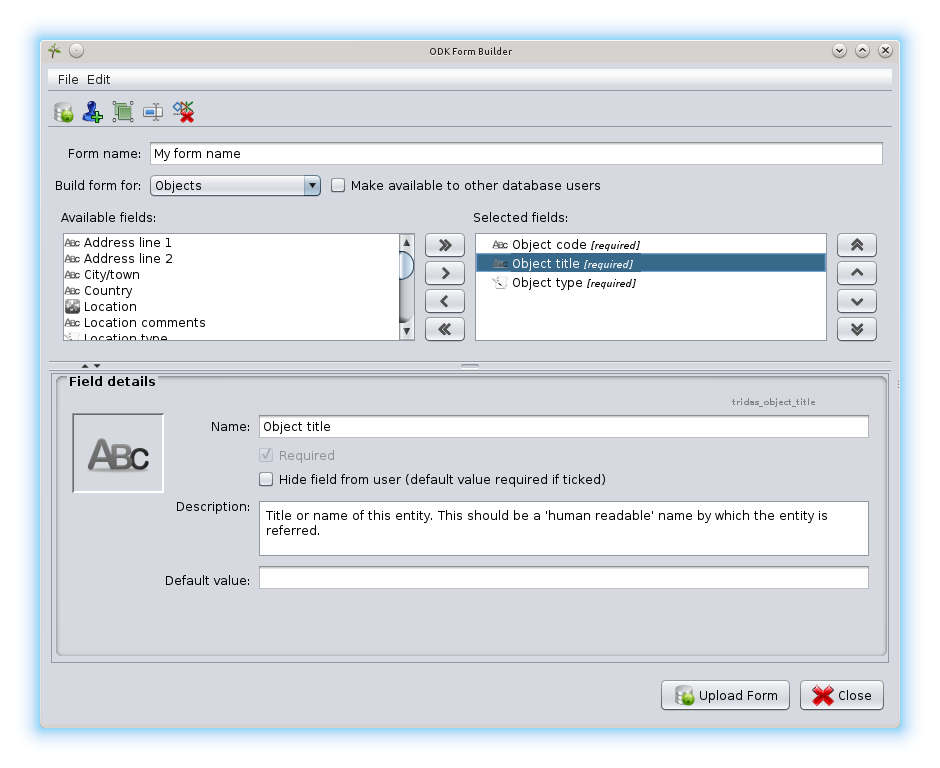
\includegraphics[width=0.6\textwidth]{Images/odkform.png}
    \caption{Screenshot of the Design ODK Form dialog.  }
    \label{fig:odkform}
 \end{figure}

The Design ODK Form dialog gives the user the ability to create two types of forms: the first for recording new objects (sites); and the second for recording elements (trees) and samples.  The user should name the form they are creating, then select the form type, and then pick all the fields that they would like to include.  Fields that are required by Tellervo and TRiDaS are pre-selected.

When you select a field you will see  it's details below depending on the data type that it stores.  You can then modifiy the field's properties.  For instance you can change the name of the field which can be useful when the person using the ODK tool in the field is not familiar with the TRiDaS terminology.  The field name `element code' might not be intuitive whereas `tree code' will be.  There is also the option to alter the help text that goes with each field.  This is another way to ensure the correct metadata is collected in the field.  It is important though that you don't change the meanings of these fields as they will be mapped back to the original TRiDaS concept when you upload the data. For instance regardless of what you choose to name the `element code' field, the contents of this field will be entered into the `element code' field in the Tellervo database.

If you know in advance the most likely information that the ODK user will want to enter you can set a default value for a field.  In this case the user can quickly confirm the entry is correct without having to enter it each time.  You also have the option of hiding a field from the ODK user.  This can be useful when you are certain of that the contents of a field.  For instance if you are collecting in `New Mexico' you might like to include the `State' field, but set the default value and hide it from the user.  This way the state is automatically recorded without the ODK user even having to confirm.

The ODK system has the ability to record a variety of data types.  Depending on the data type a different interface is shown to the data collection user.  For basic text fields, the user is shown the standard on-screen keyboard, similarly for numeric fields.  ODK has the option of using the integrated GPS receiver, in which case the user has the option of pressing a `record location' button.  It can also take photographs, video and sound recordings which can be associated as `files' in the Tellervo database. 

The final data type is the choice data type.  In this case a user is displayed a list of options from which to choose.  This is used to restrict the user to a predefined dictionary of terms (e.g.\ species, location type, object type etc).  In the form builder, choice fields like this are prepopulated with the terms used by Tellervo.  In the case of species, for instance, the list can be very long.  Selected the correct item from a long list can be slow and tedious.  The form builder tool therefore allows you to limit the list to a subset of terms.  For example, you may know before your field visit that you will collecting one of just a handful of species of trees.  Shortening the list to the likely options makes the data entry much more efficient.

All the predefined field types in the form designer correspond to the fields defined in the Tree Ring Data Standard.  If you want to collect additional metadata not covered by TRiDaS then there is the ability to add user defined fields using the blue `add user defined field' icon on the toolbar.  Note, however, that at this time these fields are ignored by Tellervo when you import your metadata into the Tellervo database.  To read data from these fields you should use the `Create CSV File' option when downloading the data using the Bulk Data Entry ODK wizard (see section \ref{txt:odkdownload}).  Alternatively you can use other ODK compatible software such as ODK Briefcase or Kobotoolbox to extract to CSV, or Excel files.

Once you have finished defining your form you need to save it either to the Tellervo server---if you are planning on using the standard wireless data transfer method---or to a file.  You can upload the form definition to the server by pressing the `Upload Form' button or alternatively if your server is not accessible over the internet you can save the form definition to an XML file on your computer by going to \menutwo{File}{Save as ODK XML file}.

If you would like to save your form definition to reuse and edit later you should use the \menutwo{File}{Save form design} option.  Note you cannot load an ODK XML form definition file within the Tellervo form designer, only the Tellervo-specific `*.odkform form design' file.


\section{ODK mobile application}
\label{txt:odktablet}

\begin{wrapfigure}{r}{0.30\textwidth}
  \begin{center}
    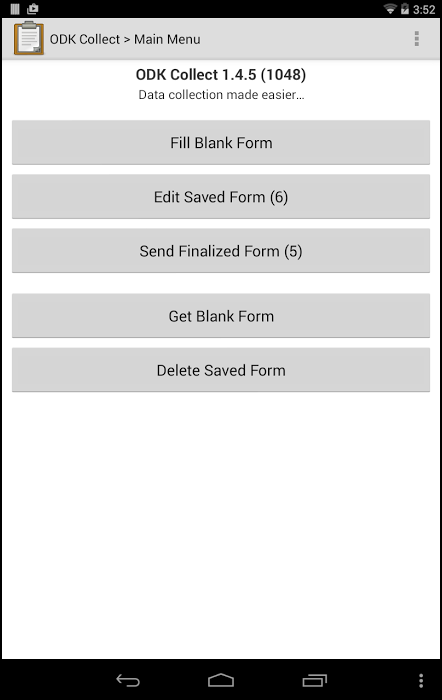
\includegraphics[width=0.26\textwidth]{Images/odkcollect.png}
  \end{center}
  \caption{Screenshot of the main screen of the ODK Collect mobile application running on an Android mobile phone.}
  \label{fig:odkcollect}
\end{wrapfigure}

Once you have generated your ODK form definition you are ready to transfer it to your mobile device.  Install the ODK Collect App from the Google Play Store as you would any other application.  

If your Tellervo server is accessible remotely then you need to configure it by going to the `general settings' page.  From here click `configure platform settings'.  The URL of your server is the same as the URL you enter when start Tellervo Desktop but with the addition of `/odk/' at the end (e.g.\ \url{http://my.ip.address/tellervo/odk/}).  Your username is your normal Tellervo username and your password is the ODK specific password that you set in the \menutwo{Adminstration}{Users and groups} page of Tellervo Desktop.  The authentication schema that ODK Collect uses is not as secure as Tellervo.  Using the same password for ODK and Tellervo would require downgrading the security on Tellervo, something we are not willing to do.  Instead a second less secure password is assigned for use with ODK Collect.  Note that this ODK password only provides limited access to load and save ODK form data to the server, it doesn't provide access to the Tellervo database.  Once you have configured your server, you can click the `Get Blank Form' button on the main menu of ODK Collect.  This will list all the ODK forms you have defined in Tellervo and allow you to transfer them to your mobile device.

If your Tellervo server is not accessible over the Internet, you will need to transfer the ODK form definitions to your device manually.  Whichever method you use, the ODK XML form definition file needs to end up in the \url{odk/forms} folder of your device.  

With your ODK form definition now installed on your mobile device you can press the `Fill Blank Form' button on the ODK Collect main menu and you should see your form in the list.  You can then create a form instance for each record that you'd like to create.  The metadata for each instance is stored as a separate XML file on your phone in the \url{odk/instance} folder, along with any additional photo, video, or sound files that you created.

\section{Importing ODK metadata into Tellervo}
\label{txt:odkdownload}
Once you have returned from the field, you can import your ODK metadata into Tellervo via the Bulk Data Entry interface (see section \ref{txt:bulkentry}).  On the Bulk Data Entry toolbar there is a 
\includegraphics[width=5mm]{Icons/22x22/odk-logo.png} button that opens up the ODK import wizard.  The wizard has a number of steps each with descriptions to walk you through the process regardless of whether you are accessing your ODK data over the network or from a local folder.  If you are doing the latter, you will need to copy the ODK form instances from your device to a local folder on your computer.  The import wizard will then access the files from there.

Once you have completed the import wizard, the Bulk Data Entry screen will be populated with all the metadata you entered in the field.  From here you can check, fix and augment the metadata before finally pressing the `import selected' button on each of the object, element and sample pages.  Once your metadata is safely imported into the Tellervo database you can then generate barcode labels for your samples using the button on the toolbar of the samples page.

\section{Deleting ODK data}
Both the ODK form definitions and form instances are by default left on the server.  If you decide you no longer want a ODK form definition any more then you can go to \menutwo{File}{Delete form designs from server} from the main Tellervo window.  Similarly you can delete form instances by going to \menutwo{File}{Delete form data from server}.  Note there is no undelete option so you need to be certain!

Both form definitions and instances are also stored on your mobile device.  To delete these too you can go to `Delete Save Form' from the main menu of ODK Collect.  From here you can delete some or all of the forms definitions and/or instances.

